\chapter{Design and Implementation}
This chapter describes the design and the implementation of the CSMA/CA simulation system.
The system is designed to model a wireless environment where the agents coordinate their access to a shared medium. 

\section{System Architecture}
The simulator is implemented as a time-driven system with four primary data structures that define the network's state:
\begin{itemize}
    \item \textbf{\texttt{Packet}} represents the unit of data. It contains metadata such as the sender ID, destination ID, and creation time.
    \item \textbf{\texttt{Node}} contains the state machine, timers, and the Reinforcement Learning (RL) agent's local knowledge.
    \item \textbf{\texttt{PacketQueue}} manages buffered packets and is implemented as a linked list.
    \item \textbf{\texttt{Simulator}} is a global structure that holds the environment parameters, node list, statistics, etc.
\end{itemize}

The simulation follows a time-slotted approach where each iteration increments the simulation clock of \texttt{t=1} (representing a \texttt{SLOT\_TIME}). In each slot, the simulator updates the state of all nodes.

\begin{lstlisting}[style=CStyle]
// Simulation loop.
for (t = 0; t <= horizon; t++) {
    for (i = 0; i < nodeNum; i++) {
        updateNode(nodes[i]);
    }
}
\end{lstlisting}
This approach is well suited for MAC protocols where the timing of backoff slots, sensing periods, and frame durations are critical.

The simulation environment is a two-dimensional monitored area.
At the beginning of each run, nodes are placed at random $(x, y)$ coordinates.\\
For example, a $7\times 5$ monitored area might be:\\
\begin{minipage}[t]{.44\textwidth}
\flushleft
\begin{verbatim}
 +---------------+
 | . . . 2 . . 6 |
 | . 0 . . . . . | The '.'
 | 8 . 5 7 . . . | indicates
 | . . . 9 . . . | the absence
 | 1 . . . . 4 3 | of nodes.
 +---------------+
\end{verbatim}
\begin{verbatim}
 Node0 => [2, 8, 5, 7] 
 Node1 => [8, 5]       
  ...  => [ ... ]       
 Node9 => [5, 7, 4]
\end{verbatim}
\textit{\texttt{Node5} and \texttt{Node8} are neighbors of \texttt{Node1}.}
\end{minipage}
\begin{minipage}[t]{.55\textwidth}
Nodes are distributed within this space, and their communication is governed by their transmission range: two nodes can communicate only if their distance is $\leq$ \texttt{RANGE} and
a collision occurs when a node is within range of multiple concurrent transmissions.
Nodes perform physical carrier sensing by detecting incoming transmissions from neighbors to determine if the channel is busy.\\
Once the nodes are randomly positioned within the monitored area, the simulator creates the network topology by generating the neighbors lists: it scans the grid and identifies all nodes located within the specified \texttt{RANGE} of each other.\\
\end{minipage}

To represent the node behavior in the simulator, we define a Finite State Machine, as illustrated in Figure \ref{fig:node-fsm}, where each state corresponds to a specific phase of the CSMA/CA protocol. The transitions are triggered by internal timers, by the status of the medium (carrier sensing), or by the arrival packets from the network. The system logic manages the transitions between the following states:
\begin{itemize}
    \item \textbf{\texttt{IDLE}:} The node has no packets to send or is waiting for a packet generation event.
    It transitions to \texttt{WAIT\_DIFS} if it has a packet in the output queue and the channel is sensed idle. If a \texttt{DATA} packet starts arriving from a neighbor, it transitions to \texttt{RECEIVING}.
    
    \item \textbf{\texttt{BACKOFF}:} The node has a packet to transmit and is decrementing its backoff counter while the channel is sensed idle.
    When the counter reaches zero, it transitions to \texttt{TRANSMITTING} to send its \texttt{DATA} packet.
    
    \item \textbf{\texttt{TRANSMITTING}:} The node is currently sending a \texttt{DATA} or \texttt{ACK} packet.
    Upon completion, if the packet was \texttt{DATA}, the node moves to \texttt{WAIT\_ACK}. If it was an \texttt{ACK}, it returns to \texttt{IDLE}.
    
    \item \textbf{\texttt{RECEIVING}:} The node is receiving a \texttt{DATA} or \texttt{ACK} packet.
    If a \texttt{DATA} packet is successfully received, the node transitions to \texttt{WAIT\_SIFS} to prepare an acknowledgement. Otherwise it returns to \texttt{IDLE}.
    
    \item \textbf{\texttt{WAIT\_ACK}:} After transmission, the node waits, for a given period of time, an \texttt{ACK} packet from the receiver.
    If a valid \texttt{ACK} is detected, it transitions to \texttt{RECEIVING}. If the \texttt{ACK\_TIMEOUT} is hit, it assumes a collision or loss has occurred and, it returns to \texttt{IDLE} to schedule a retransmission. (Here it also updates the Contention Window or RL values.)
    
    \item \textbf{\texttt{WAIT\_DIFS}} and \textbf{\texttt{WAIT\_SIFS}:} Waiting periods required by the CSMA/CA protocol.
    After \texttt{DIFS}, if the channel becomes busy, it returns to \texttt{IDLE} to defer transmission. If the timer expires while the channel is idle, it moves to \texttt{BACKOFF}.
    After \texttt{SIFS}, once the timer expires, the node transitions to \texttt{TRANSMITTING}.
\end{itemize}

\begin{figure}[ht]
    \centering
    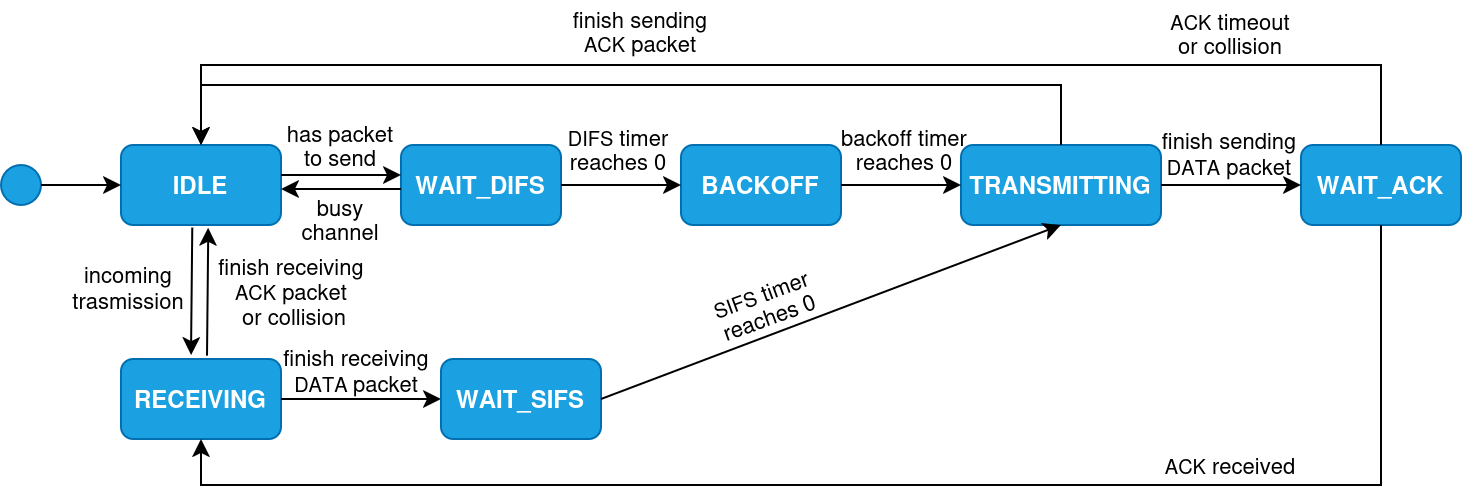
\includegraphics[width=1\linewidth]{figures/node-fsm.png}
    \caption{Finite State Machine of a node in the CSMA/CA simulator.}
    \label{fig:node-fsm}
\end{figure}

\section{Communication Flow}
The communication process follows the standard CSMA/CA protocol. The flow of a single transmission attempt is:
\begin{itemize}
    \item \textbf{Packet generation:} In each time slot, a node generates a \texttt{DATA} packet with a probability \texttt{GEN\_PROB} and places it in its output queue.
    
    \item \textbf{Carrier sensing:} The node performs a physical carrier sense by checking if any neighbors are currently in the \texttt{TRANSMITTING} state. If the channel is idle, it waits for a \texttt{DIFS} period. If the channel becomes busy during this time, the process restarts.
    
    \item \textbf{Backoff:} Nodes pick a random timer from their Contention Window (\texttt{CW}).    This backoff counter decrements only when the channel is idle.
    
    \item \textbf{Data transmission:} When the backoff counter reaches zero, the node broadcasts its \texttt{DATA} packet to all neighbors. Here we model a half-duplex system: if a node is \texttt{TRANSMITTING}, it cannot "hear" incoming packets and will automatically discard any arrivals.
    
    \item \textbf{Acknowledgment (ACK):} Upon successful reception of a \texttt{DATA} packet, the destination waits for a \texttt{SIFS} interval and then sends an \texttt{ACK} packet back to the sender. A transmission is considered successful only if the sender receives this \texttt{ACK} before a timeout; otherwise, it doubles its \texttt{CW} and attempts a retransmission.
\end{itemize}

Each node manages its internal data flow using two distinct packet queues: 
\begin{itemize} 
    \item \textbf{Output Queue:} This acts as a buffer for packets the node wants to send. It stores locally generated \texttt{DATA} packets and high-priority \texttt{ACK} responses. \texttt{ACK}s are moved to the front of this queue to ensure they are sent immediately after the \texttt{SIFS} period. 
    
    \item \textbf{Input Queue:} This acts as a reception buffer where the network delivers packets. During each slot, the simulator checks this queue. If it contains multiple packets simultaneously, it indicates a collision. If only one packet is present, the node begins the \texttt{RECEIVING} process. 
\end{itemize}

To avoid the computational cost of deep-copying packets for every neighbor, the simulator uses a reference counting mechanism.
As illustrated in Figure \ref{fig:communication-flow}, when a node sends a packet, it doesn't create $n$ copies for $n$ neighbors.
Instead, it creates one packet object and gives each neighbor a reference to it. 

For every neighbor that successfully adds the packet to its input queue, the packet's \texttt{refcount} is increased by one. Once a node is done with the packet (either by processing it or discarding it due to a collision), it calls \texttt{releasePacket}, which decreases the count. The memory occupied by the packet is only actually deleted from the system when the \texttt{refcount} reaches zero, meaning that no more nodes are using it. 

\begin{figure}[ht]
    \centering
    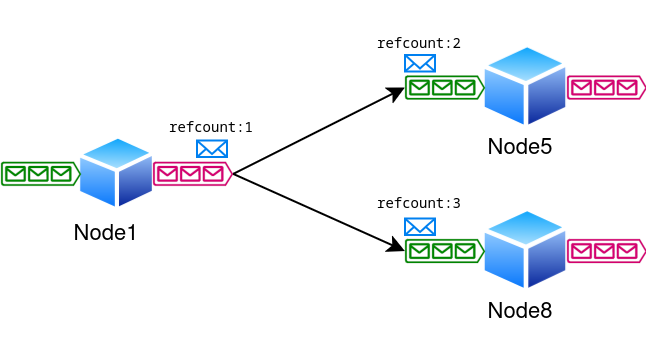
\includegraphics[width=0.6\linewidth]{figures/communication-flow.png}
    \caption{Representation of the communication flow between nodes.}
    \label{fig:communication-flow}
\end{figure}

\section{Adaptive RL Policy}
The core innovation of this simulator is the transition from the static contention window of standard CSMA/CA to an Adaptive RL-based policy. This approach treats the selection of the contention window as a decision-making problem, allowing nodes to optimize their behavior in real-time based on environmental feedback.

\begin{itemize}
    \item \textbf{Actions:} The agent selects from a set of $K$ arms, where each arm corresponds to a specific CW value (e.g., $CW\in\{15,31,…,1023$\}).
    
    \item \textbf{Reward function:} After every transmission attempt, the environment provides a reward. A successful transmission (ACK received) yields a positive reward, while a collision or timeout results in a negative reward.

    \item \textbf{Update rule:} The agent maintains an estimated value (Q-value) for each arm. These are updated using an incremental update rule with a constant step-size $\alpha$, allowing the node to prioritize recent network conditions over old data:
    \begin{equation*}
    Q(A)\leftarrow Q(A)+\alpha[Reward-Q(A)]
    \end{equation*}

    \item \textbf{Policy:} An $\epsilon$-greedy strategy is used to balance exploration (trying new CW values) and exploitation (using the best CW value found so 
    far).
\end{itemize}
 
\begin{lstlisting}[style=CStyle]
/* Select the next contention window using the Epsilon-Greedy strategy. */
void selectAction(Node *node) {
    // Explore. Choose a random arm.
    if (rand() < epsilon) {
        action = rand() % ARMS_NUM;
    }
    // Eploit. Choose the arm with the highest Q-value.
    else {
        int bestArm = 0;
        double maxQ = node->qValues[0];
        for (int i = 0; i < ARMS_NUM; i++) {
            if (node->qValues[i] > maxQ) {
                maxQ = node->qValues[i];
                bestArm = i;
            }
        }
        action = bestArm;
    }
}
\end{lstlisting}

\section{Performance Metrics}
To evaluate the efficiency of the autonomous RL policy against the standard protocol, the simulator tracks global performance metrics. 
These metrics are computed at the end of each simulation run:
\begin{itemize}
    \item \textbf{Packet Delivery Ratio (PDR):} Measures the reliability of the network by calculating the percentage of generated packets that are successfully delivered and acknowledged. It is computed as:
    \begin{equation*}
        PDR=\frac{Packets Acked} {Packets Generated}
    \end{equation*}
    A higher PDR indicates a robust protocol that effectively manages contention and minimizes packet loss.
    
    \item \textbf{Throughput:} Represents the effective data rate of the network, calculated as the number of successfully received packets over the total simulation time.
    \begin{equation*}
        Throughput=\frac{Packets Received}{Total Simulation Time (ticks)}
    \end{equation*}
    Throughput reflects how efficiently the medium is utilized; the RL policy aims to maximize this metric by selecting optimal Contention Windows that reduce idle time.
    
    \item \textbf{Collision Rate:} Identifies the impact of simultaneous transmissions. It is the ratio of detected collisions to the total number of packets sent.
    \begin{equation*}
        Collision Rate=\frac{Collisions}{Packets Sent}
    \end{equation*}
    A collision is recorded when a node is within range of multiple concurrent transmissions. Reducing this rate is a primary goal of the RL agent's backoff strategy.
    
    \item \textbf{Average Latency:} This tracks the time elapsed from the moment a packet is generated to the moment it is successfully acknowledged.
    \begin{equation*}
        Avg Latency=\frac{\sum(Time of ACK Reception-Packet Creation Time)}{Total Packets Acked}   
    \end{equation*}
\end{itemize}

Because our wireless environments is stochastic due to random node placement and randomized backoff timers, the simulator performs multiple independent runs. Then each performance metric tracks the mean and variance across these runs to allow for comparison between the "Standard" and the "Adaptive CW" models.